\documentclass[a4paper,14pt]{extarticle}

\usepackage[a4paper,top=20mm,bottom=20mm,left=30mm,right=10mm]{geometry}
\usepackage[T1,T2A]{fontenc}
\usepackage[utf8]{inputenc}
\usepackage[russian]{babel}
\usepackage{indentfirst}
\usepackage{titlesec}
\usepackage{graphicx}
\usepackage{verbatim}
\usepackage{fancyvrb}

\renewcommand{\baselinestretch}{1.3}
\titleformat{\section}{\normalsize\bfseries}{\thesection}{1em}{}
\titleformat{\subsection}{\normalsize\bfseries}{\thesection}{1em}{}
\setlength{\parindent}{12.5mm}

\begin{document}

  \newpage\thispagestyle{empty}
  \begin{center}
    \MakeUppercase{
      Министерство науки и высшего образования Российской Федерации\\
      Федеральное государственное бюджетное образовательное учреждение высшего образования\\
      <<Вятский Государственный Университет>>\\
    }
    Институт математики и информационных систем\\
    Факультет автоматики и вычислительной техники\\
    Кафедра электронных вычислительных машин
  \end{center}
  \vfill

  \begin{center}
    Отчет по лабораторной работе №6\\
    по дисциплине\\
    <<Программирование>>\\
  \end{center}
  \vfill

  \noindent
  \begin{tabular}{ll}
    Выполнил студент гр. ИВТб-1301-05-00 \hspace{5mm} &
    \rule[-1mm]{25mm}{0.10mm}\,/Макаров С.А./\\
    
    Руководитель зав. кафедры ЭВМ & \rule[-1mm]{25mm}{0.10mm}\,/Долженкова М.Л./\\
  \end{tabular}

  \vfill
  \begin{center}
    Киров 2025
  \end{center}

  \newpage
  \section*{Цель}
  Цель лабораторной работы: изучение структуры и принципов организации программных модулей, закрепление навыков работы с динамической памятью, получение базовых навыков организации работы в режиме командной строки.

  \section*{Задание}
  \begin{enumerate}
    \item Написать программу для работы со структурой данных <<Очередь>>.
    \item Структура данных должна быть реализована на основе динамической памяти.
    \item Структура данных (поля и методы) должна быть описана в отдельном модуле.
    \item Работа со структурой должна осуществляться в режиме командной строки (с реализацией автодополнения и истории команд). Предусмотреть наглядную визуализацию содержимого структуры.
  \end{enumerate}

  \pagebreak
  \section*{Решение}

  \begin{figure}[h]
    \centering
    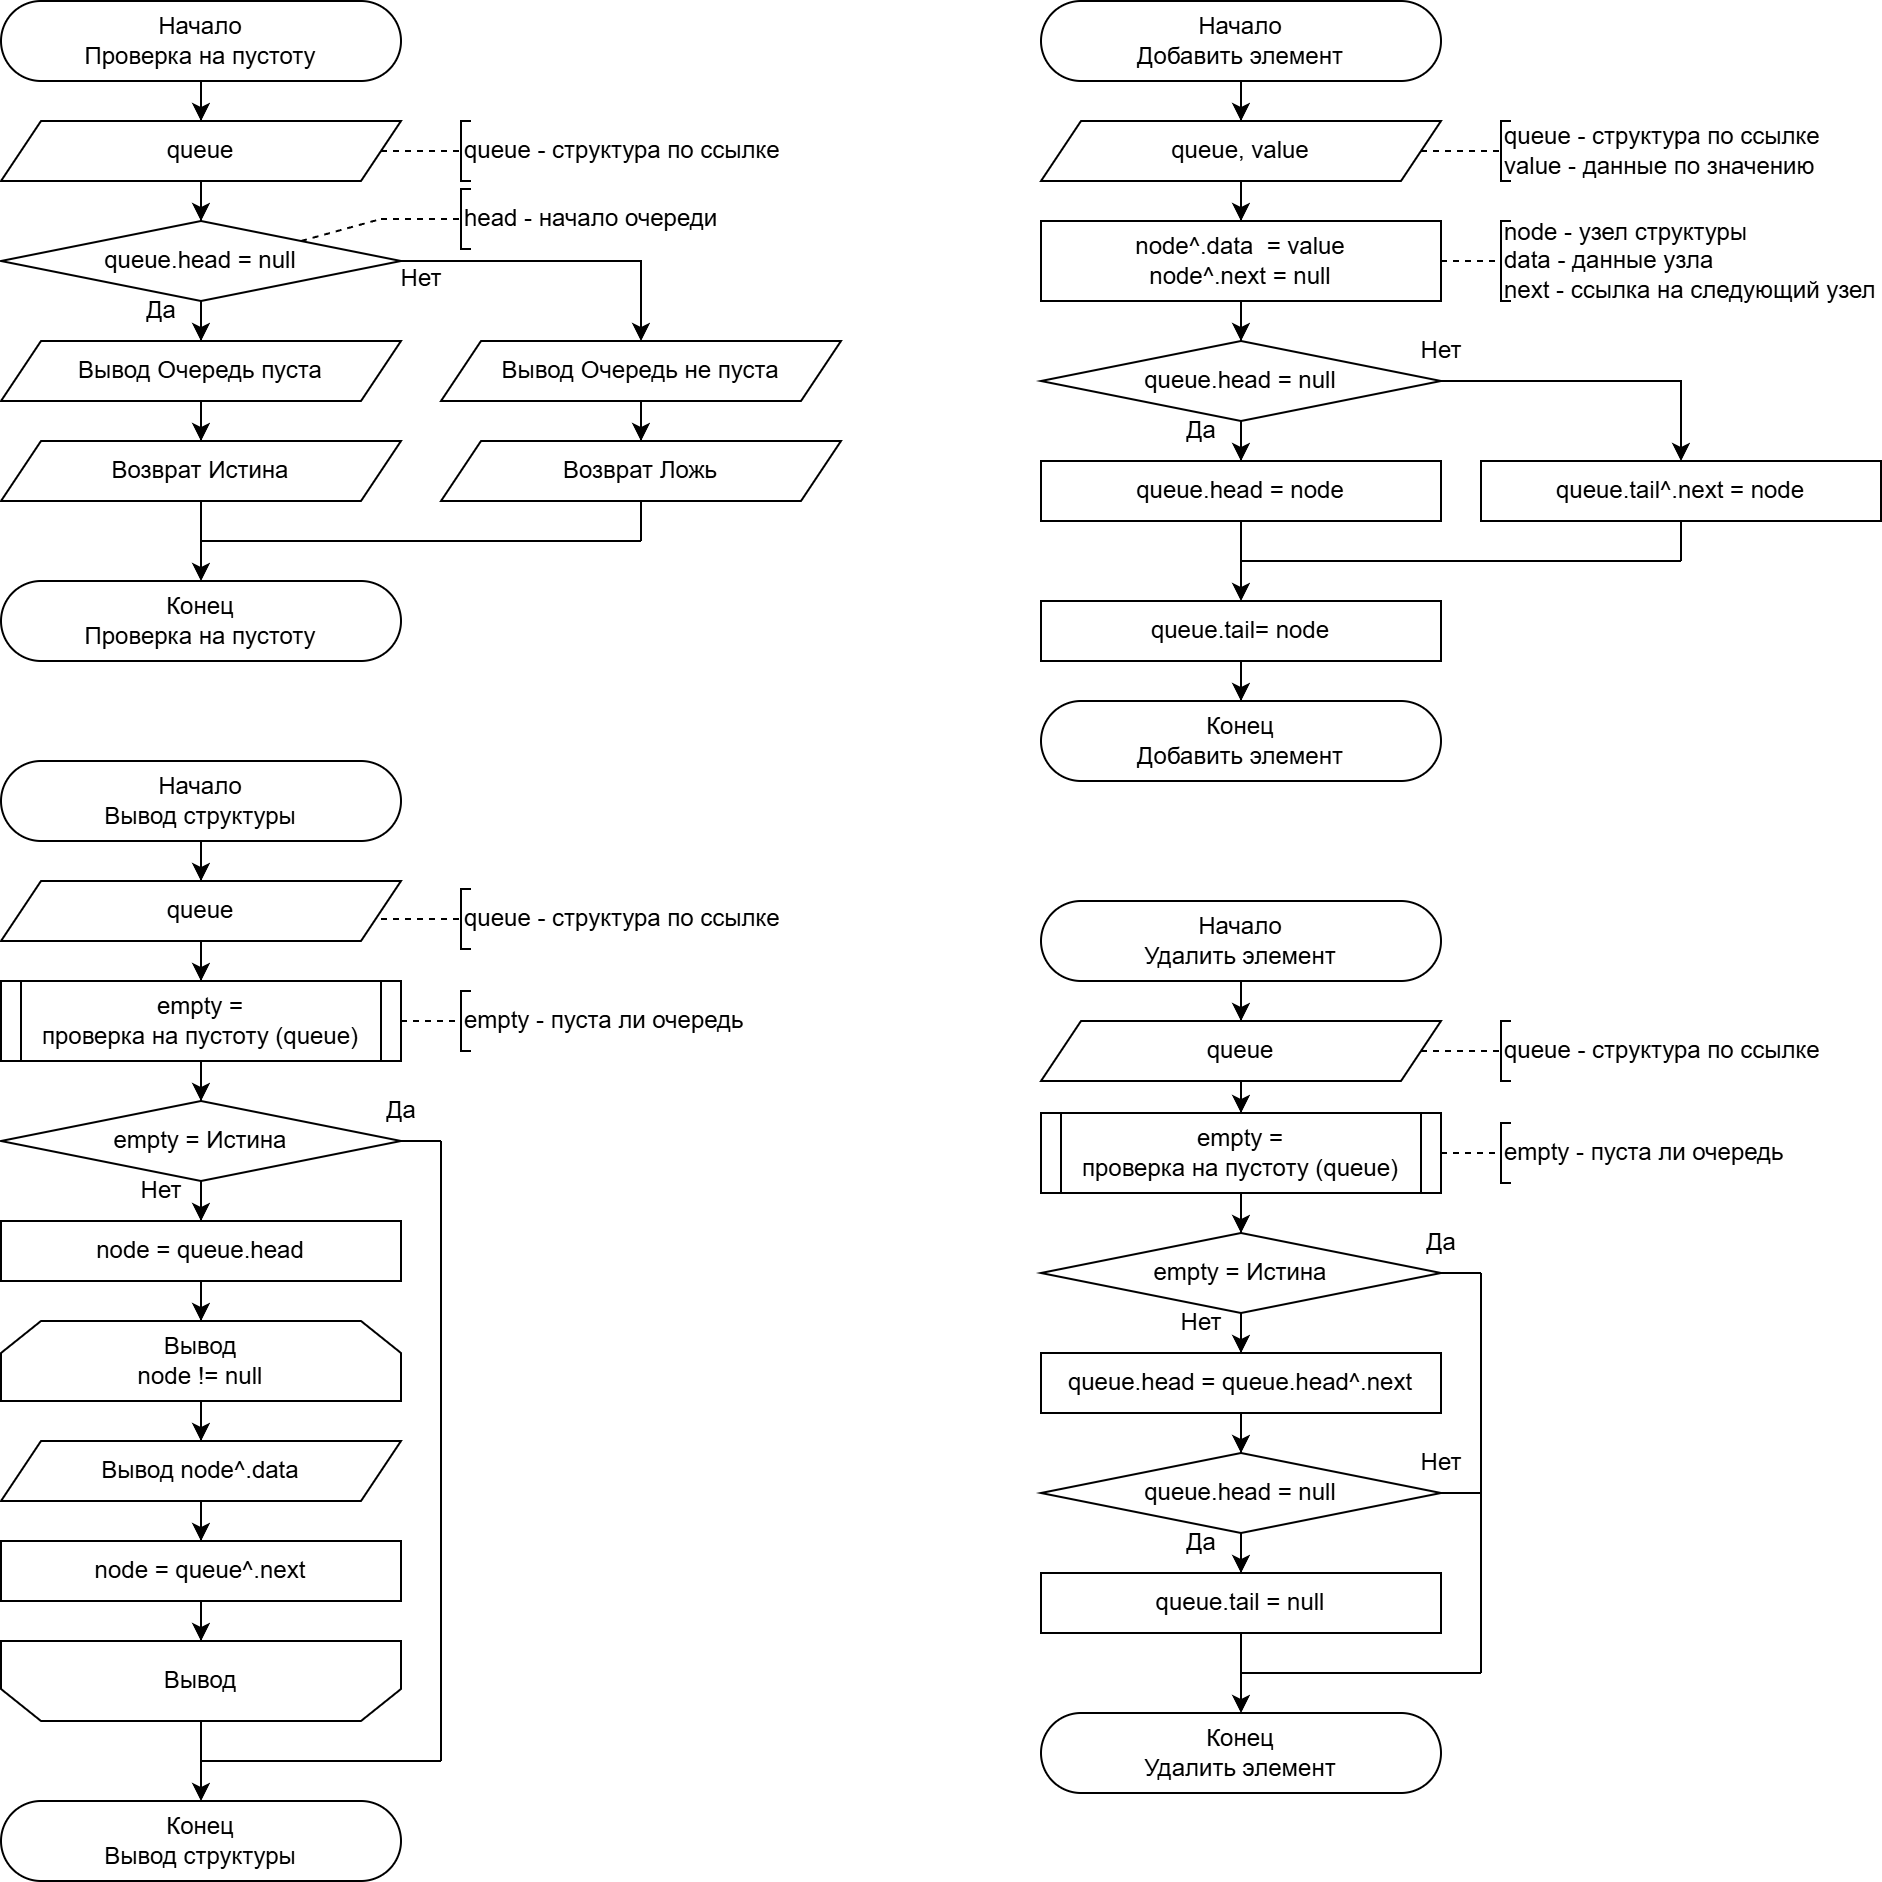
\includegraphics[width=1\linewidth]{images/s-1}
  \end{figure}
  \begin{center}
    Рисунок 1 – Схемы алгоритмов проверки на пустоту, вывода структуры, удаления и добвления элемента
  \end{center}

  \pagebreak

  \begin{figure}[h]
    \centering
    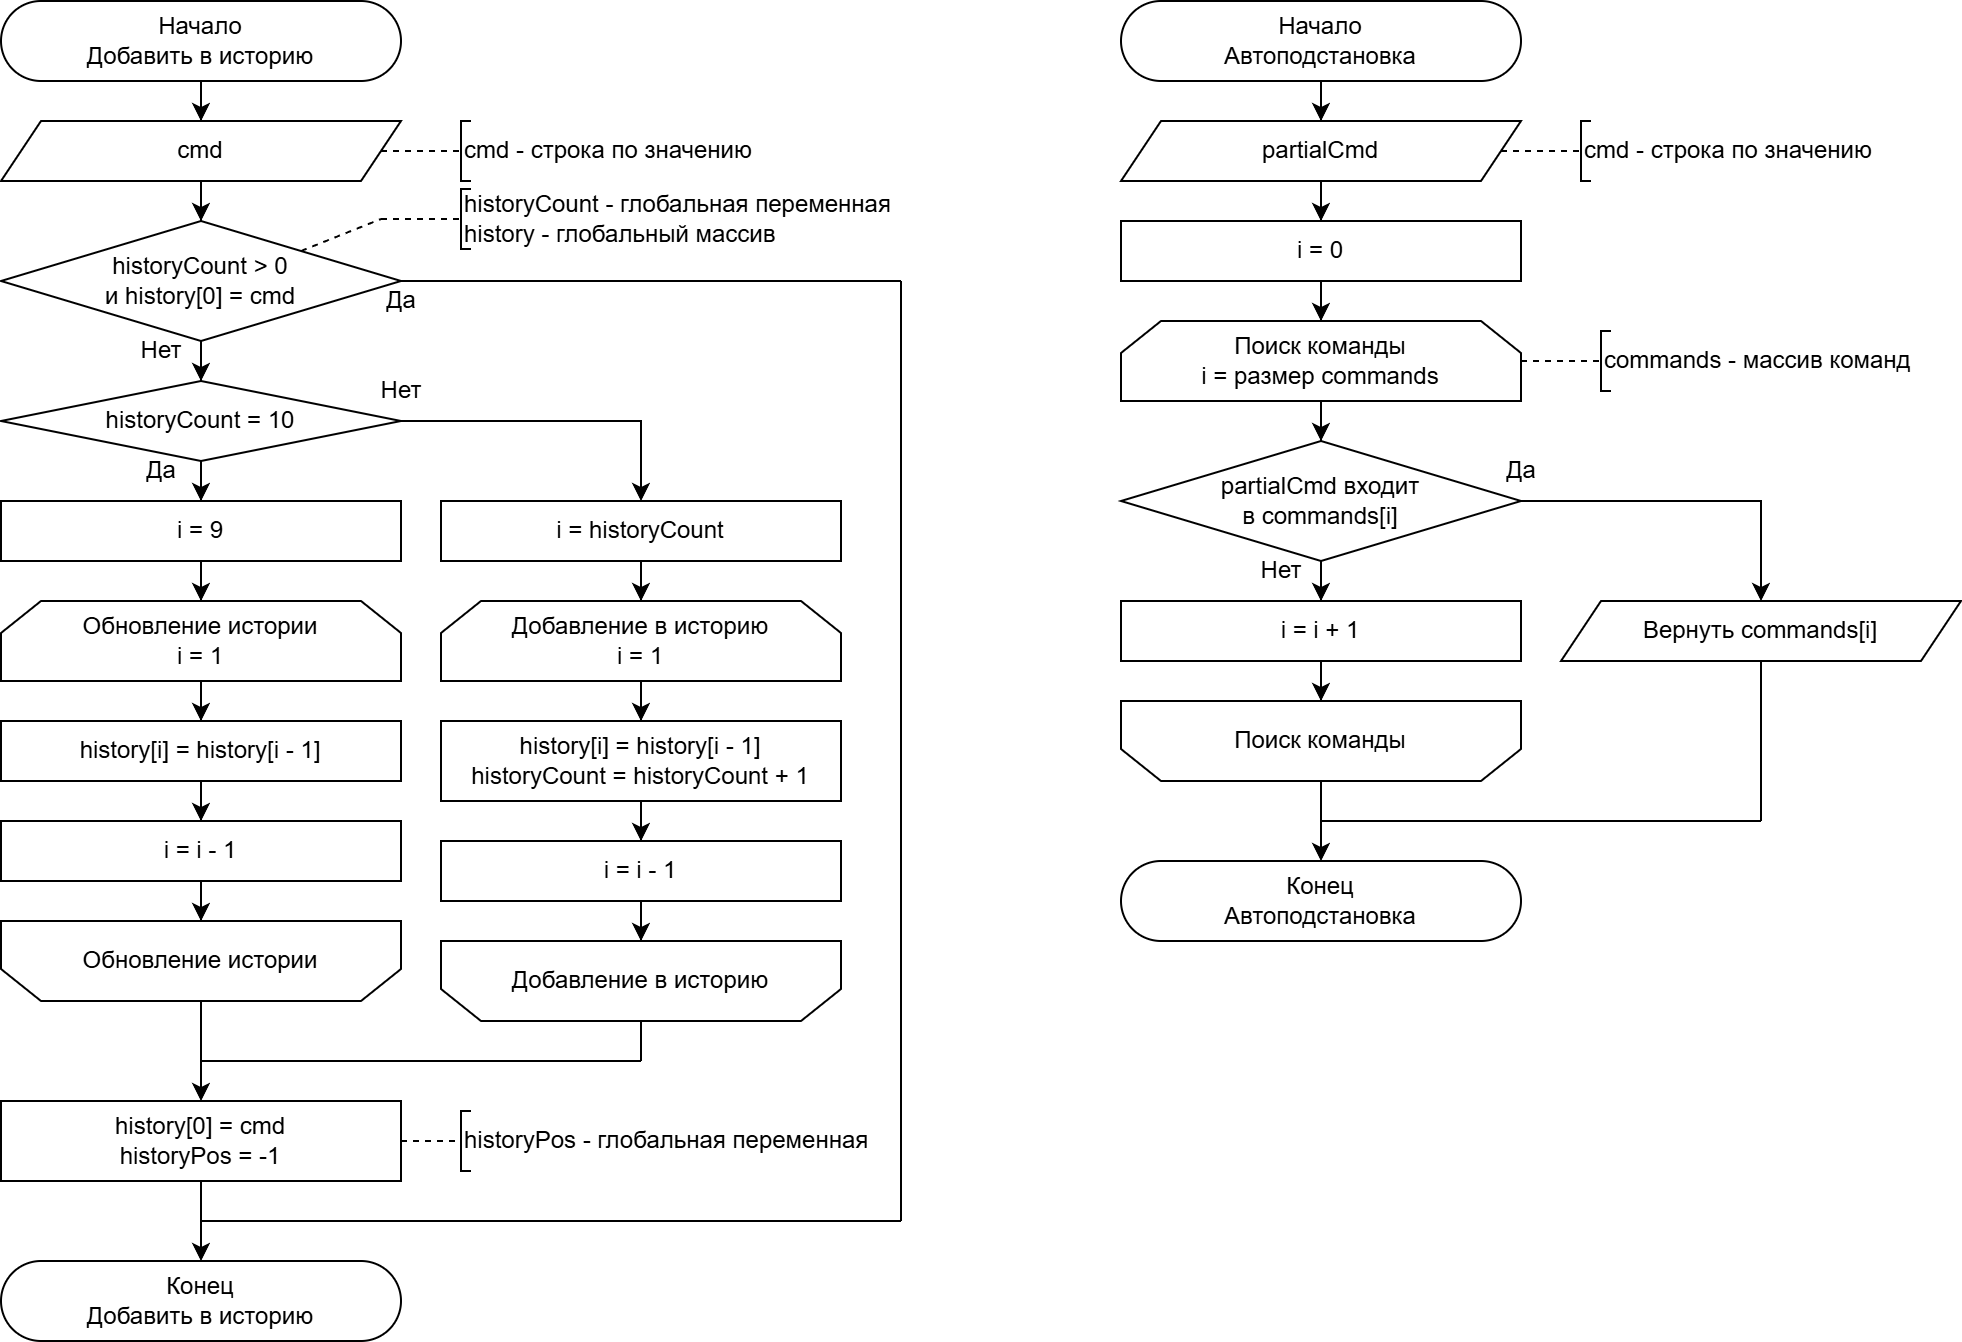
\includegraphics[width=1\linewidth]{images/s-2}
  \end{figure}
  \begin{center}
    Рисунок 2 – Схемы алгоритмов добавления в историю, автоподстановки
  \end{center}

  \pagebreak

  \begin{figure}[h]
    \centering
    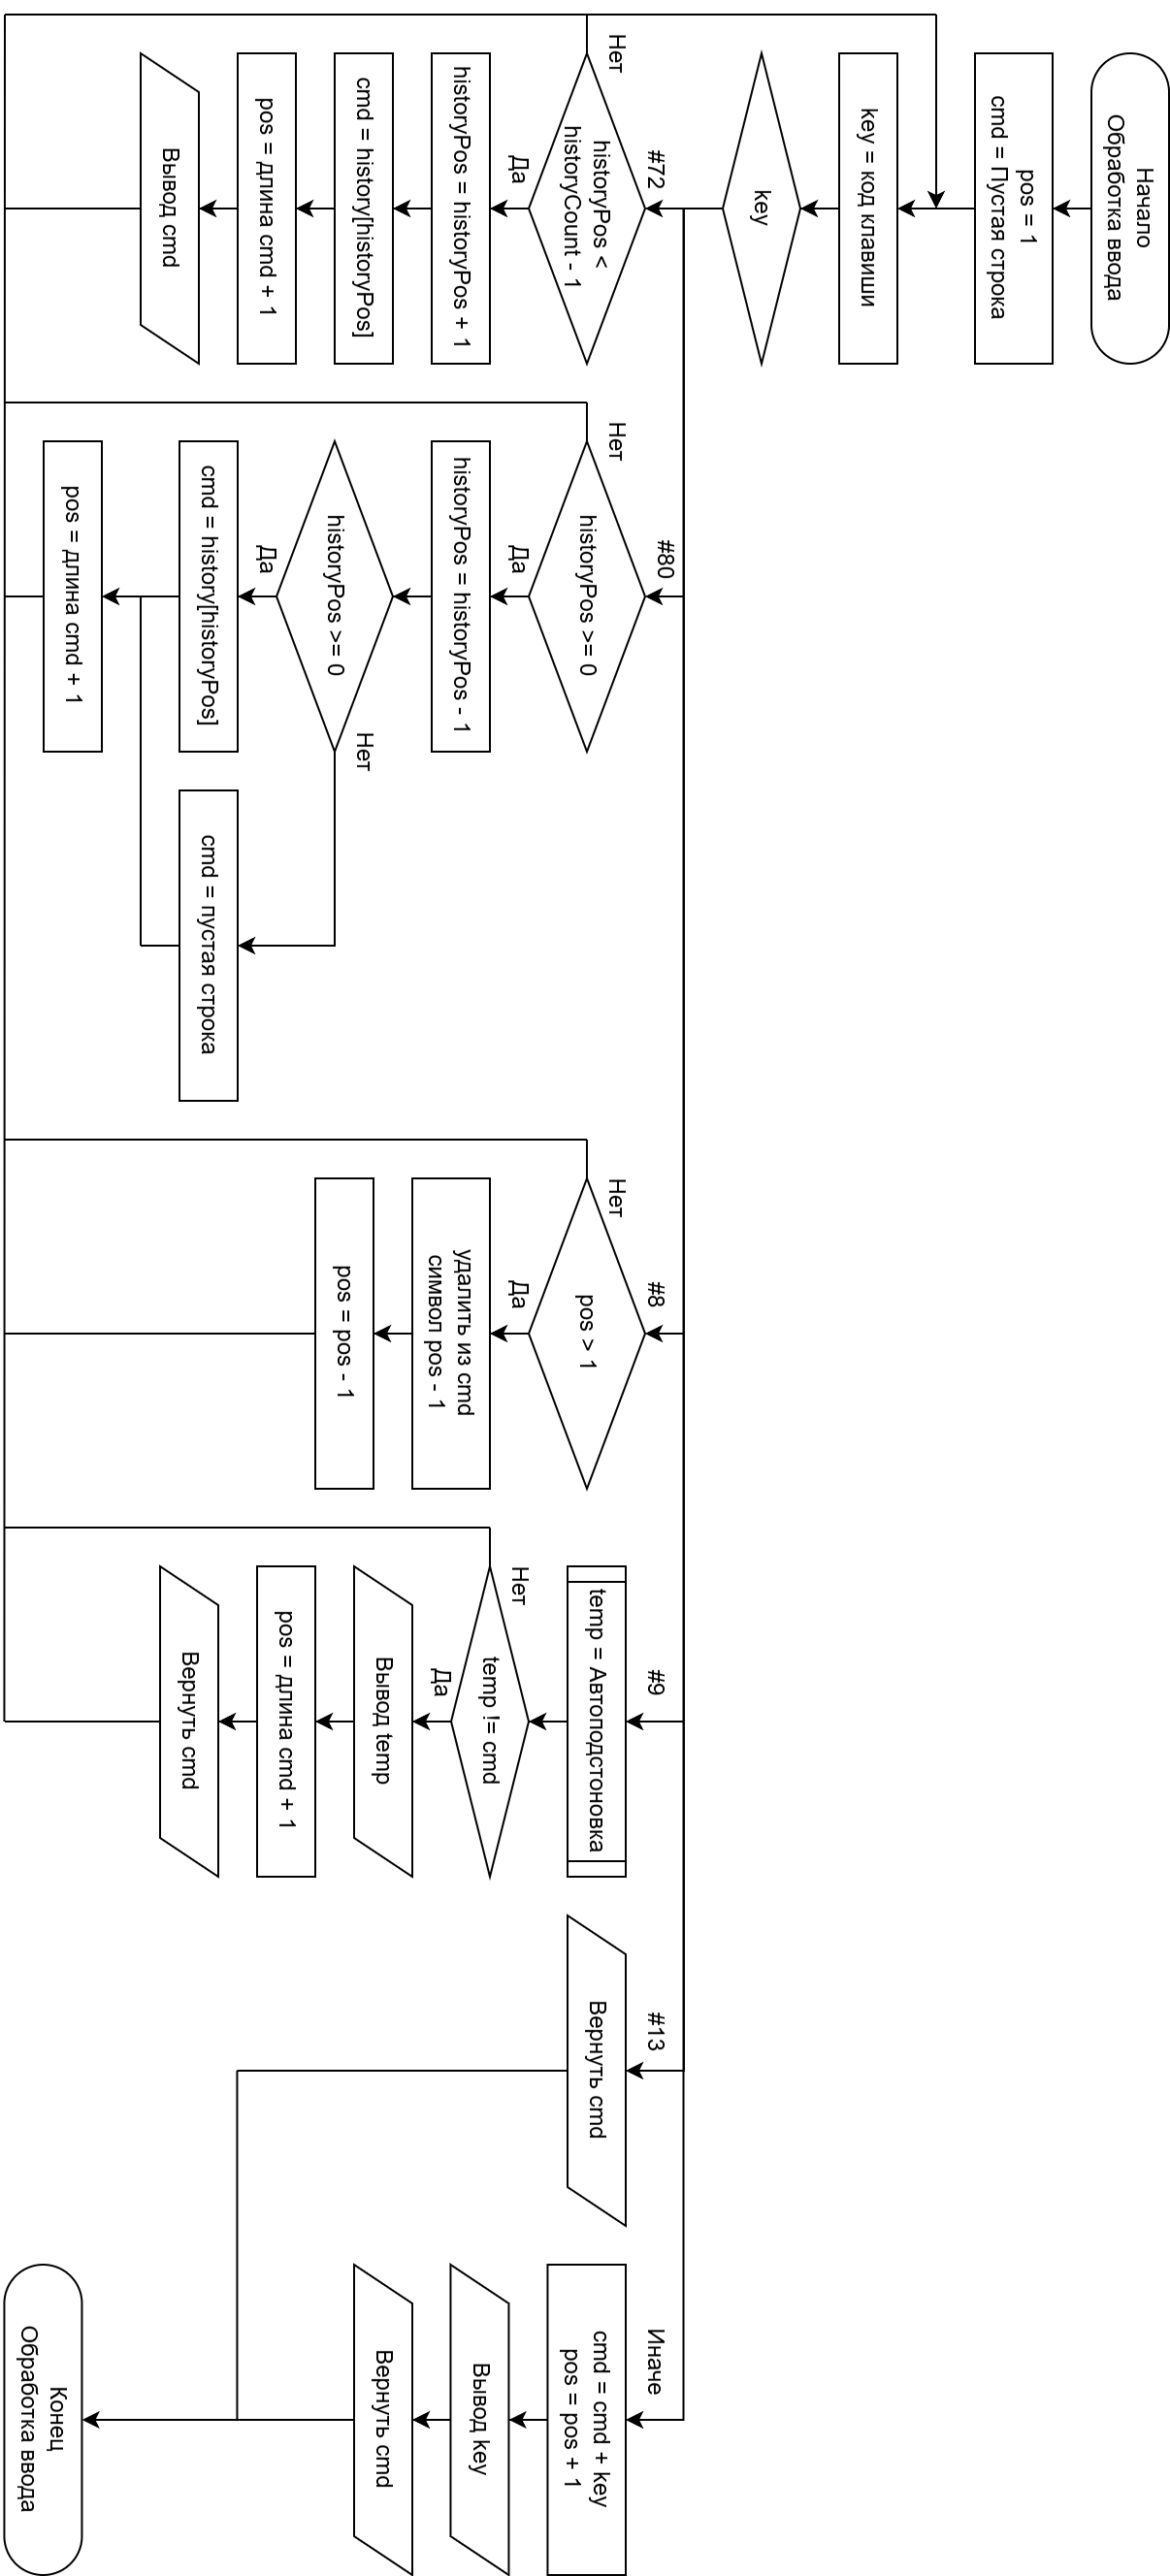
\includegraphics[width=0.535\linewidth]{images/s-3}
  \end{figure}
  \begin{center}
    Рисунок 3 – Схема алгоритма обработки ввода
  \end{center}

  \pagebreak

  \begin{figure}[h]
    \centering
    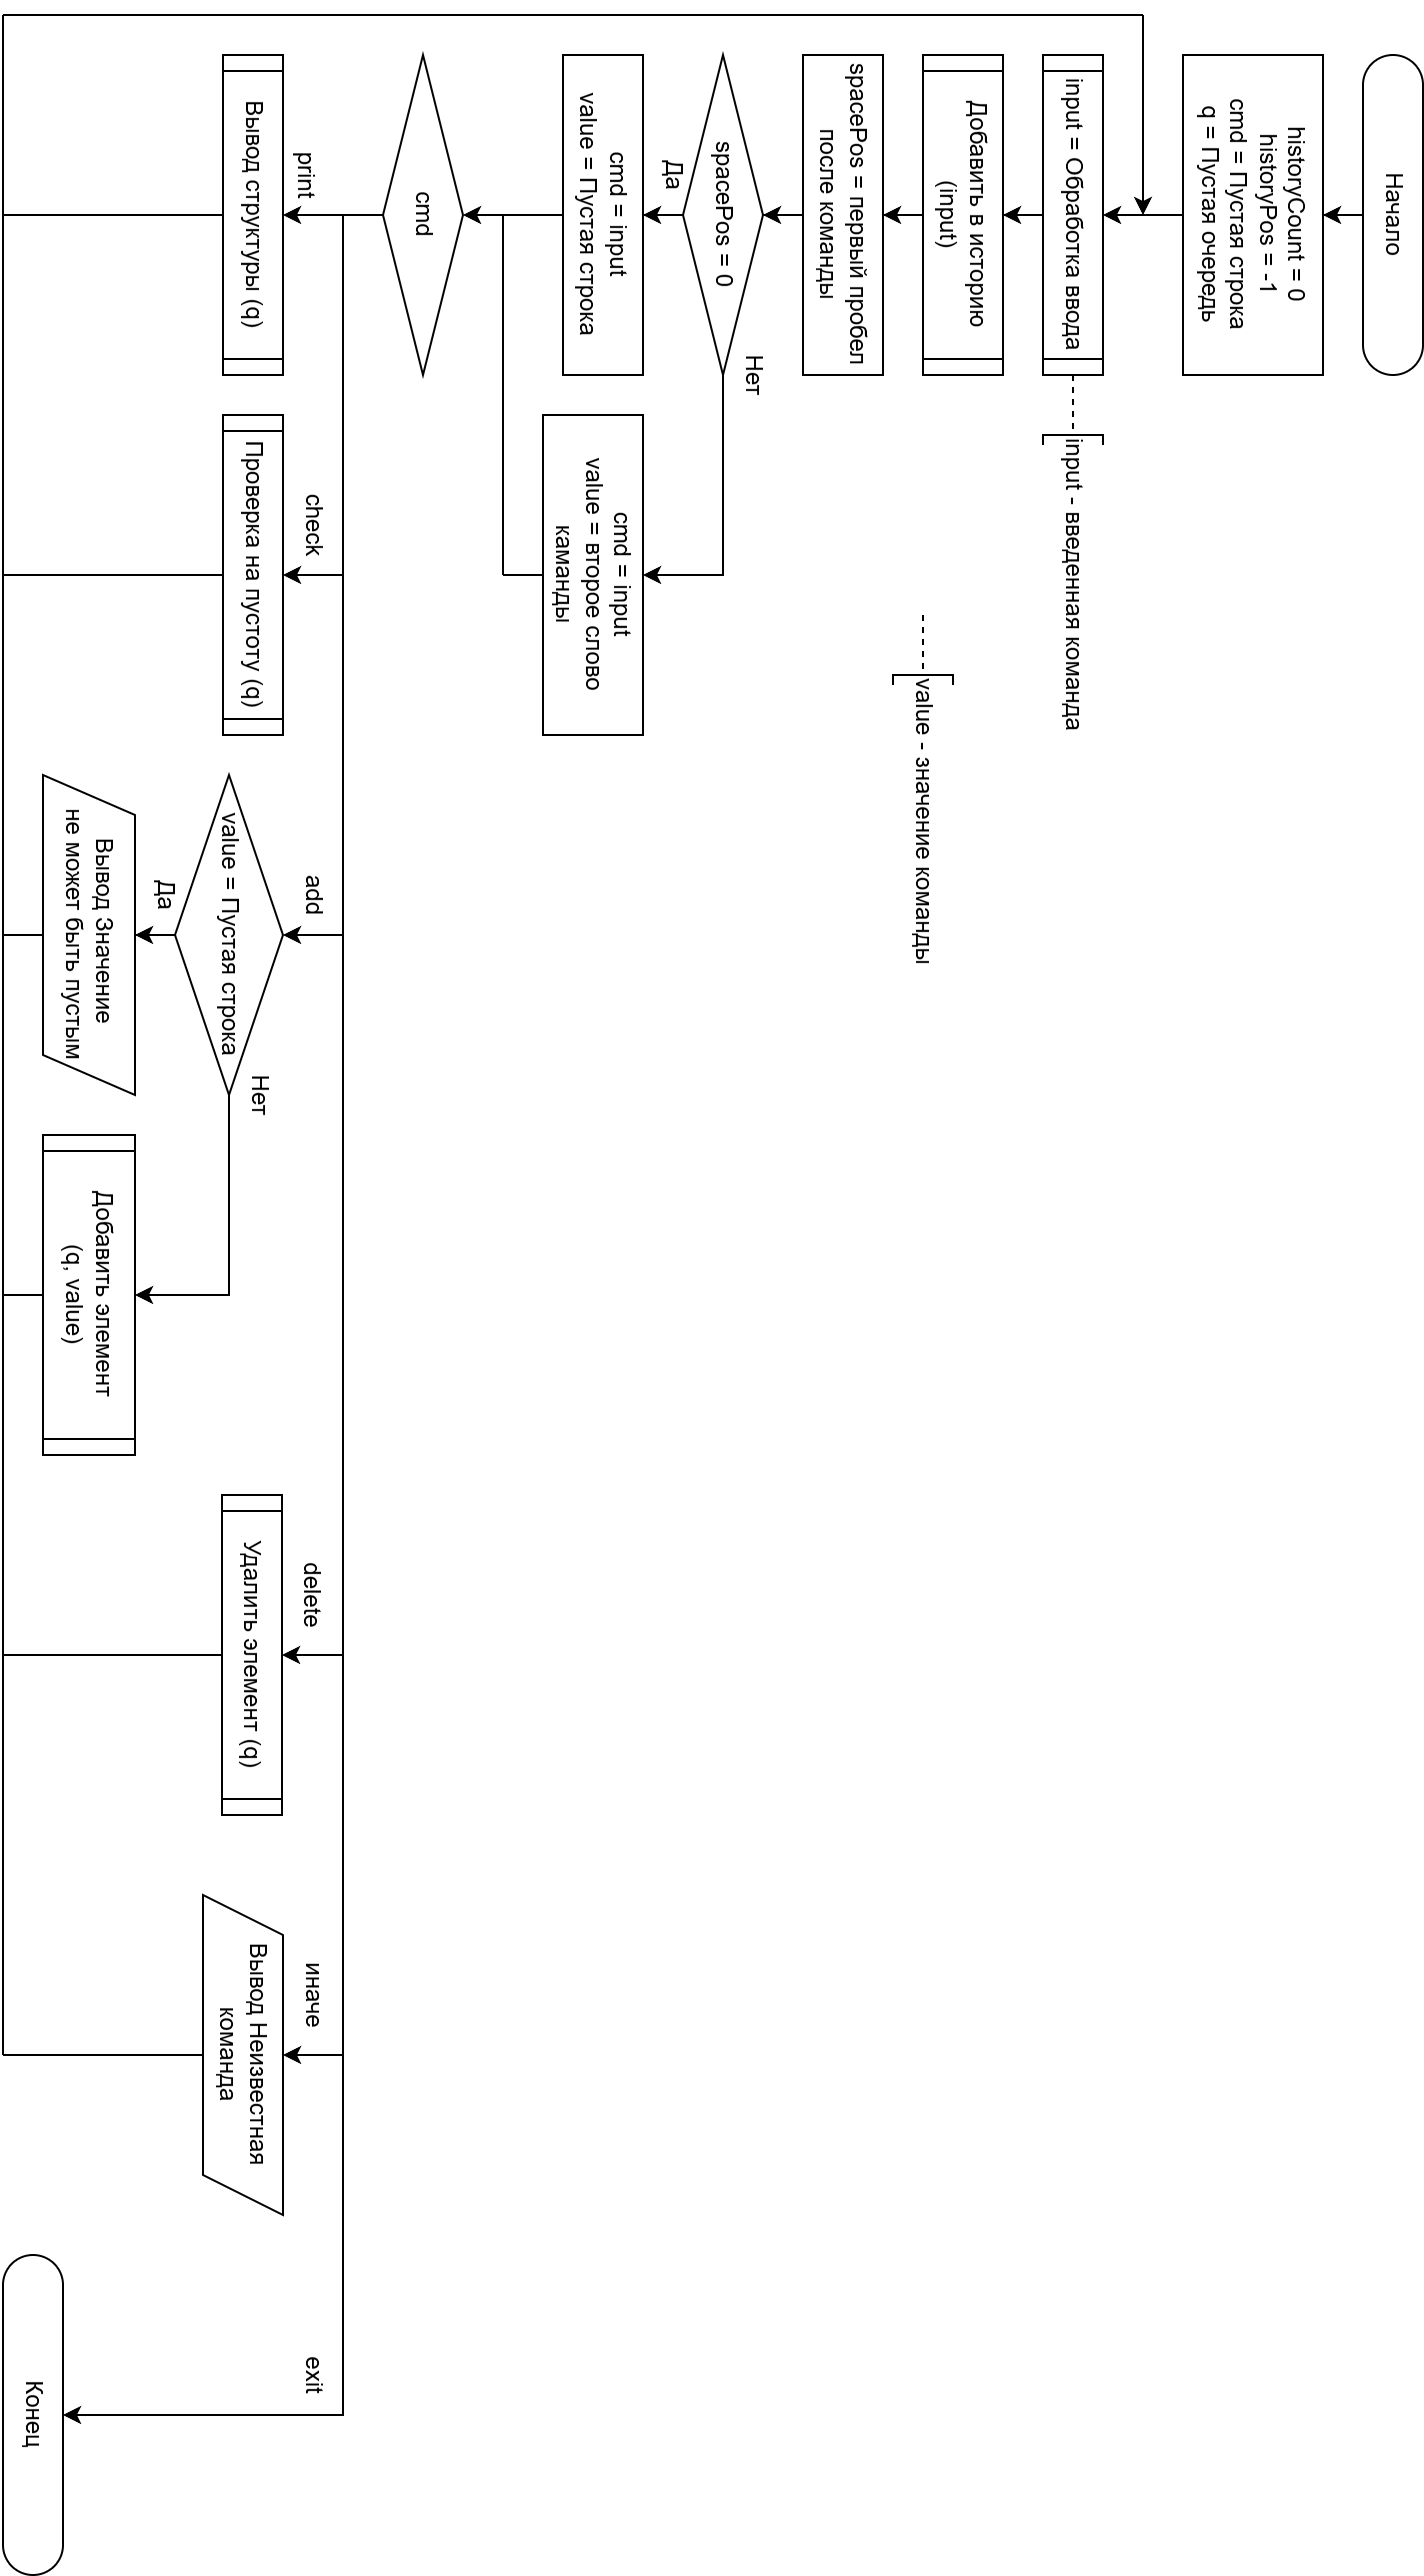
\includegraphics[width=0.65\linewidth]{images/s-4}
  \end{figure}
  \begin{center}
    Рисунок 4 – Схема алгоритма программы
  \end{center}

  \pagebreak

  Исходный код модуля для структуры <<Очередь>> представлен ниже:

  \noindent
  \begin{Verbatim}[tabsize=4,fontsize=\small]
{$codepage UTF8}
unit Queue;
interface
  type
    PNode = ^TNode;
    TNode = record
      data: string;
      next: PNode;
    end;
    TQueue = record
      head, tail: PNode;
    end;
  function check(var queue: TQueue): boolean;
  procedure init(var queue: TQueue);
  procedure push(var queue: TQueue; value: string);
  procedure pop(var queue: TQueue);
  procedure print(var queue: TQueue);
implementation
  function check(var queue: TQueue): boolean;
  begin
    if queue.head = nil then
    begin
      writeln('Очередь пуста');
      exit(true);
    end;
    writeln('Очередь не пуста');
    check := false;
  end;
  procedure init(var queue: TQueue);
  begin
    queue.head := nil;
    queue.tail := nil;
  end;
  procedure push(var queue: TQueue; value: string);
  var
    node: PNode;
  begin
    new(node);
    node^.data := value;
    node^.next := nil;
    if queue.head = nil then
      queue.head := node
    else
      queue.tail^.next := node;

    queue.tail := node;
  end;
  procedure pop(var queue: TQueue);
  begin
    if check(queue) then exit;
    queue.head := queue.head^.next;
    if queue.head = nil then
      queue.tail := nil;
  end;
  procedure print(var queue: TQueue);
  var
    node: PNode;
  begin
    if check(queue) then
      exit;
    node := queue.head;
    while node <> nil do
    begin
      write(node^.data, ' ');
      node := node^.next;
    end;
    writeln();
  end;
end.
  \end{Verbatim}

  Исходный код главного модуля представлен ниже:

  \noindent
  \begin{Verbatim}[tabsize=4,fontsize=\small]
{$codepage UTF8}
uses
  SysUtils, Crt, Queue;
const
  MAX_HISTORY = 10;
  COMMANDS: array[0..5] of string = ('help', 'exit', 'print', 
    'check', 'add', 'delete');
var
  q: TQueue;
  running: boolean;
  input, cmd, value: string;
  spacePos: integer;
  history: array[0..MAX_HISTORY - 1] of string;
  historyCount, historyPos: integer;
procedure showHelp();
begin
  writeln();
  writeln('  Список команд:');
  writeln('------------------------------------------------');
  writeln('  help - список команд');
  writeln('  exit - выход из консоли');
  writeln('  print - вывод очереди');
  writeln('  check - проверка очереди на пустоту');
  writeln('  add <значение> - добавить элемент в очередь');
  writeln('  delete - удалить элемент из очереди');
  writeln();
end;
procedure addToHistory(cmd: string);
var
  i: integer;
begin
  if cmd = '' then exit;
  if (historyCount > 0) and (history[0] = cmd) then exit;
  if historyCount = MAX_HISTORY then
  begin
    for i := MAX_HISTORY - 1 downto 1 do
      history[i] := history[i - 1];
  end
  else
  begin
    for i := historyCount downto 1 do
      history[i] := history[i - 1];
    historyCount := historyCount + 1;
  end;
  history[0] := cmd;
  historyPos := -1;
end;
function autoComplete(partialCmd: string): string;
var
  i: integer;
begin
  if partialCmd = '' then exit;

  for i := 0 to length(COMMANDS) - 1 do
  begin
    if pos(partialCmd, COMMANDS[i]) = 1 then
      autoComplete := COMMANDS[i]
  end;
end;
function getConsoleInput(): string;
var
  key: char;
  cmd, temp: string;
  pos, i: integer;
begin
  cmd := '';
  pos := 1;
  repeat
    key := ReadKey();
    case key of
      #0:
        begin
          key := ReadKey();
          case key of
            #72:
              if historyPos < historyCount - 1 then
              begin
                historyPos := historyPos + 1;
                for i := 1 to length(cmd) do
                  write(#8' '#8);
                cmd := history[historyPos];
                pos := length(cmd) + 1;
                write(cmd);
              end;
            #80:
              if historyPos >= 0 then
              begin
                historyPos := historyPos - 1;
                for i := 1 to length(cmd) do
                  write(#8' '#8);
                if historyPos >= 0 then
                  cmd := history[historyPos]
                else
                  cmd := '';
                pos := length(cmd) + 1;
                write(cmd);
              end;
          end;
        end;
      #8:
        begin
          if pos > 1 then
          begin
            delete(cmd, pos - 1, 1);
            pos := pos - 1;
            write(#8' '#8);
          end;
        end;
      #9:
        begin
          temp := autoComplete(cmd);
          if temp <> cmd then
          begin
            for i := 1 to length(cmd) do
              write(#8' '#8);
            write(temp);
            cmd := temp;
            pos := length(cmd) + 1;
            getConsoleInput := cmd;
          end;
        end;
      #13:
        begin
          writeln();
          getConsoleInput := cmd;
          exit;
        end;
      else
        begin
          insert(key, cmd, pos);
          pos := pos + 1;
          write(key);
          getConsoleInput := cmd;
        end;
    end;
  until false;
end;
begin
  init(q);
  running := true;
  historyCount := 0;
  historyPos := -1;
  clrscr();
  showHelp();
  while running do
  begin
    write('> ');
    input := trim(getConsoleInput());
    if input = '' then continue;
    addToHistory(input);
    spacePos := pos(' ', input);
    if spacePos = 0 then
    begin
      cmd := input;
      value := '';
    end
    else
    begin
      cmd := copy(input, 1, spacePos - 1);
      value := trim(copy(input, spacePos + 1, length(input)));
    end;
    case cmd of
      'help': showHelp();
      'exit': running := false;
      'print': print(q);
      'check': check(q);
      'add':
        begin
          if value = '' then
            writeln('Значение не может быть пустым')
          else
            push(q, value);
        end;
      'delete': pop(q);
      else
        writeln('Неизвестная команда: ', cmd, ' Введите "help" для справки');
    end;
  end;
end.
  \end{Verbatim}

  \section*{Вывод}
  В ходе выполнения лабораторной работы были изучены структуры и принципы организации программных модулей, закреплены навыки работы с динамической памятью. Также получены базовые навыки организации работы в режиме командной строки.

\end{document}